\documentclass[10pt]{article}
\usepackage{amsmath}
\usepackage{amssymb}
\usepackage{amsthm}
\usepackage{cases}

\usepackage{graphicx}
\usepackage{float}

\title{Projet automatique}
\author{David Castro et Anatole Hernot}
\date{16 décembre 2021}

\begin{document}
\maketitle
\theoremstyle{definition}

\newcommand{\inv}[1]{\frac{1}{#1}}

\section{Système en boucle ouverte}

\subsection*{Équation d'état}

État $X = (x, v = \dot x, \theta, q = \dot{\theta})$, $u$, l'entrée de commande, $d$, l'entrée de perturbation, $x_m$ et $\theta_m$ les mesures et $x_m$ la sortie à commander.

\vspace{10px}

\noindent On a alors :  $\dot X = \begin{bmatrix} \dot x \\ \dot v \\ \dot \theta \\ \dot q \end{bmatrix} =
\begin{bmatrix} v \\ x q^2 + g \sin \theta \\ q \\ \frac{gx \cos \theta + u + d - 2xqv}{\alpha + x^2} \end{bmatrix}$
avec $\alpha = \frac{J}{m}$.

\subsection*{Point d'équilibre}

\[ \begin{cases} \bar v = 0 \\ \bar x \bar q^2 + g \sin \bar{\theta}  = 0 \\ \bar q = 0 \\ \frac{g \bar x \cos \bar{\theta} + \bar u + \bar d - 2 \bar x \bar q \bar v}{\alpha + \bar x^2} = 0 \end{cases} \]

\[ \begin{cases} \bar v = 0 \\ \sin \bar{\theta}  = 0 \\ \bar q = 0 \\ g \bar x \cos \bar{\theta} + \bar u + \bar d = 0 \end{cases} \]

\vspace{10px}

\noindent Il y a donc deux points d'équilibre : $\left( - \frac{\bar u + \bar d}{g}, 0, 0, 0 \right)$ et $\left( \frac{\bar u + \bar d}{g}, 0, \pi, 0 \right)$.

\subsection*{Linéarisation}

On linéarise au premier point d'équilibre car si on atteint $\theta = \pi$, cela signifie que le rail s'est retourné et donc que la bille est tombée.

\vspace{10px}

\noindent Le système linéarisé tangent en ce point est :

\begin{align}
\delta \dot X &=
	\begin{bmatrix} 
		\delta v \\
		2 \bar x \bar q \delta q + g \delta \theta \\
		\delta q \\
		\frac{g \delta x + \delta u + \delta d - 2 \bar q \bar v \delta x}{\alpha + \bar x^2} - 2 \bar x \delta x \frac{g \bar x + \bar u + \bar d}{\left( \alpha + \bar x^2 \right)^2}
	\end{bmatrix} \notag \\
	&= \begin{bmatrix} 
		\delta v \\
		g \delta \theta \\
		\delta q \\
		\frac{g \delta x + \delta u + \delta d}{\alpha + \bar x^2}
	\end{bmatrix}
	\text{le second terme de $\delta \dot q$ s'annulant par définition de $\bar x$}
	\notag \\
	&= \underbrace{
	\begin{bmatrix}
		0 & 1 & 0 & 0 \\
		0 & 0 & g & 0 \\
		0 & 0 & 0 & 1 \\
		\frac{g}{\alpha + \bar x^2} & 0 & 0 & 0
	\end{bmatrix}
	}_{A}
	\delta X
	+
	\underbrace{
	\begin{bmatrix}
		0 & 0 \\
		0 & 0 \\
		0 & 0 \\
		\frac{1}{\alpha + \bar x^2} & \frac{1}{\alpha + \bar x^2}
	\end{bmatrix}
	}_{B}
	\delta e \notag
\end{align}

\subsection*{Calcul des valeurs propres}

\begin{align}
	\chi_A (X) &=
	\begin{vmatrix}
		X & -1 & 0 & 0 \\
		0 & X & -g & 0 \\
		0 & 0 & X & -1 \\
		- \frac{g}{\alpha + \bar x^2} & 0 & 0 & X
	\end{vmatrix} \notag \\
	&= X \begin{vmatrix}
		X & -g & 0 \\
		0 & X & -1 \\
		0 & 0 & X
	\end{vmatrix} + 
	\frac{g}{\alpha + \bar x^2} \begin{vmatrix}
		-1 & 0 & 0 \\
		X & -g & 0 \\
		0 & X & -1
	\end{vmatrix} \notag \\
	&= X^4 - \frac{g^2}{\alpha + \bar x^2} \notag
\end{align}

\noindent D'où $\mathrm{Sp} \left( A \right) = \{ \beta ; - \beta ; \beta i ; - \beta i\}$ avec
$\beta =  \sqrt[4]{\frac{g^2}{\alpha + \bar x^2}}  > 0$. Donc le système linéarisé est ue-instable.

\section{Étude préliminaire en boucle fermée}

\subsection*{Ajout d'un contrôleur sur $x$}

Pour tâcher de rendre le système stable au point d'équilibre, on pose un contrôleur proportionnel-dérivé
au niveau de la position :

\[
	\delta u = - k ( \delta x_m - \delta x_r ) - k_d \delta \dot x_m
\]

\noindent En notant $x_r$ la consigne de position. Alors en négligeant $\nu_x$ le bruit de mesure de $x$,
on a $x_m = x$ et $\dot x_m = v$ donc :

\begin{align}
\delta \dot X &=
	\begin{bmatrix}
		0 & 1 & 0 & 0 \\
		0 & 0 & g & 0 \\
		0 & 0 & 0 & 1 \\
		\frac{g}{\alpha + \bar x^2} & 0 & 0 & 0
	\end{bmatrix}
	\delta X
	+
	\begin{bmatrix}
		0 & 0 \\
		0 & 0 \\
		0 & 0 \\
		\frac{1}{\alpha + \bar x^2} & \frac{1}{\alpha + \bar x^2}
	\end{bmatrix}
	\begin{bmatrix}
		- k ( \delta x - \delta x_r ) - k_d \delta v \\ \delta d
	\end{bmatrix}
	\notag \\
	&= \underbrace{
	\begin{bmatrix}
		0 & 1 & 0 & 0 \\
		0 & 0 & g & 0 \\
		0 & 0 & 0 & 1 \\
		\frac{g - k}{\alpha + \bar x^2} & - \frac{k_d}{\alpha + \bar x^2} & 0 & 0
	\end{bmatrix}
	}_{A'}
	\delta X
	+
	\begin{bmatrix}
		0 & 0 \\
		0 & 0 \\
		0 & 0 \\
		\frac{1}{\alpha + \bar x^2} & \frac{1}{\alpha + \bar x^2}
	\end{bmatrix}
	\begin{bmatrix}
		k \delta x_r \\ \delta d
	\end{bmatrix}
	\notag
\end{align}

\noindent On obtient alors le polynôme caractéristique :

\begin{align}
	\chi_{A'} (X) &=
	\begin{vmatrix}
		X & -1 & 0 & 0 \\
		0 & X & -g & 0 \\
		0 & 0 & X & -1 \\
		- \frac{g - k}{\alpha + \bar x^2} & \frac{k_d}{\alpha + \bar x^2} & 0 & X
	\end{vmatrix} \notag \\
	&= X \begin{vmatrix}
		X & -g & 0 \\
		0 & X & -1 \\
		\frac{k_d}{\alpha + \bar x^2} & 0 & X
	\end{vmatrix} + 
	\frac{g - k}{\alpha + \bar x^2} \begin{vmatrix}
		-1 & 0 & 0 \\
		X & -g & 0 \\
		0 & X & -1
	\end{vmatrix} \notag \\
	&= X \left( X^3 + \frac{g k_d}{\alpha + \bar x^2} \right) - \frac{g (g - k)}{\alpha + \bar x^2} \notag \\
	&= X^4 + \frac{g k_d}{\alpha + \bar x^2} X - \frac{g (g - k)}{\alpha + \bar x^2} \notag
\end{align}

\noindent Le coefficient d'ordre $3$, c'est-à-dire en l'occurrence $n - 1$ où $n = 4$ est le degré du polynôme,
est nul. Le critère de Routh donne donc directement que le système linéarisé n'est pas stable car $A'$
n'a pas toutes ses valeurs propres à partie réelle strictement positive.

\subsection*{Ajout d'un contrôleur sur $\theta$}

On pose cette fois le contrôleur proportionnel-dérivé au niveau de $\theta$ :

\[
	\delta u = - k ( \delta \theta_m - \delta \theta_r ) - k_d \delta \dot \theta_m
\]

\noindent En notant $\theta_r$ la consigne de position. Alors en négligeant $\nu_{\theta}$ le bruit de mesure de $\theta$ :

\begin{align}
\delta \dot X &=
	\begin{bmatrix}
		0 & 1 & 0 & 0 \\
		0 & 0 & g & 0 \\
		0 & 0 & 0 & 1 \\
		\frac{g}{\alpha + \bar x^2} & 0 & 0 & 0
	\end{bmatrix}
	\delta X
	+
	\begin{bmatrix}
		0 & 0 \\
		0 & 0 \\
		0 & 0 \\
		\frac{1}{\alpha + \bar x^2} & \frac{1}{\alpha + \bar x^2}
	\end{bmatrix}
	\begin{bmatrix}
		- k ( \delta \theta - \delta \theta_r ) - k_d \delta q \\ \delta d
	\end{bmatrix}
	\notag \\
	&= \underbrace{
	\begin{bmatrix}
		0 & 1 & 0 & 0 \\
		0 & 0 & g & 0 \\
		0 & 0 & 0 & 1 \\
		\frac{g}{\alpha + \bar x^2} & 0 & - \frac{k}{\alpha + \bar x^2} & - \frac{k_d}{\alpha + \bar x^2}
	\end{bmatrix}
	}_{A''}
	\delta X
	+
	\begin{bmatrix}
		0 & 0 \\
		0 & 0 \\
		0 & 0 \\
		\frac{1}{\alpha + \bar x^2} & \frac{1}{\alpha + \bar x^2}
	\end{bmatrix}
	\begin{bmatrix}
		k \delta \theta_r \\ \delta d
	\end{bmatrix}
	\notag
\end{align}

\noindent On obtient alors le polynôme caractéristique :

\begin{align}
	\chi_{A''} (X) &=
	\begin{vmatrix}
		X & -1 & 0 & 0 \\
		0 & X & -g & 0 \\
		0 & 0 & X & -1 \\
		- \frac{g}{\alpha + \bar x^2} & 0 & \frac{k}{\alpha + \bar x^2} & X + \frac{k_d}{\alpha + \bar x^2}
	\end{vmatrix} \notag \\
	&= X \begin{vmatrix}
		X & -g & 0 \\
		0 & X & -1 \\
		0 & \frac{k}{\alpha + \bar x^2} & X + \frac{k_d}{\alpha + \bar x^2}
	\end{vmatrix} + 
	\frac{g}{\alpha + \bar x^2} \begin{vmatrix}
		-1 & 0 & 0 \\
		X & -g & 0 \\
		0 & X & -1
	\end{vmatrix} \notag \\
	&= X \left[ X^2 \left( X + \frac{k_d}{\alpha + \bar x^2} \right) + \frac{k}{\alpha + \bar x^2} X \right]
		- \frac{g^2}{\alpha + \bar x^2} \notag \\
	&= X^4 + \frac{k_d}{\alpha + \bar x^2} X^3 +  \frac{k}{\alpha + \bar x^2} X^2
		- \frac{g^2}{\alpha + \bar x^2} \notag
\end{align}

\noindent On applique le critère de Routh :

\begin{align}
	\begin{vmatrix}
		\frac{k_d}{\alpha + \bar x^2} & 1 & 0 \\
		0 & \frac{k}{\alpha + \bar x^2} &\frac{k_d}{\alpha + \bar x^2} \\
		0 & - \frac{g^2}{\alpha + \bar x^2} & 0
	\end{vmatrix}
	&> 0 \tag{\text{condition} 3} \\
	\begin{vmatrix}
		\frac{k_d}{\alpha + \bar x^2} & 1 & 0 & 0 \\
		0 & \frac{k}{\alpha + \bar x^2} &\frac{k_d}{\alpha + \bar x^2} & 1 \\
		0 & - \frac{g^2}{\alpha + \bar x^2} & 0 & \frac{gk}{\alpha + \bar x^2} \\
		0 & 0 & 0 & - \frac{g^2}{\alpha + \bar x^2}
	\end{vmatrix}
	&> 0 \tag{\text{condition} 4}
\end{align}

\vspace{10px}

\noindent En notant $D$ le premier déterminant, on obtient en développant le second déterminant selon la dernière
ligne le système :

\[
	\begin{cases}
		D > 0 \\
		- \frac{g^2}{\alpha + \bar x^2} D > 0
	\end{cases}
\]

\newpage

\noindent C'est impossible donc $A''$ admet des valeurs propres à partie réelle négative et le système linéarisé n'est
pas stable.

\subsection*{Conclusion sur la question 1}

\fbox{
	\begin{minipage}{0.96\textwidth}
		Il n'est donc pas possible de commander le système en utilisant une seule des deux mesures :
		dans les deux cas, on n'obtient pas un système stable. Il va donc falloir utiliser les deux.
	\end{minipage}
}

\section{Système en boucle fermé}

\newcommand{\kt}{k_{\theta}}
\newcommand{\kdx}{k^d_x}
\newcommand{\kdt}{k^d_{\theta}}
\newcommand{\fact}[1]{\frac{g #1 }{\alpha + \bar x^2}} % 1 nombre d'arguments

\subsection*{Bouclage du système}

\noindent Pour ce faire, on distingue deux sous-parties du système :

\begin{itemize}
	\item $\theta$ est considérée comme une variable rapide car c'est sur elle qu'influe directement la commande $u$ ;
	\item $x$ est considéré comme une variable lente car ses variations sont consécutives à celles de $\theta$ et
	pas directement à la commande.
\end{itemize}

\noindent On va donc contrôler le système rapide par un un PD et le système lent par un PID, comme suit :

\[
	\begin{cases}
		\theta_r = - k_i \rho - k x_m - k_d \dot x_m \\
		\dot \rho = x_m - x_r \\
		u = - \lambda ( \theta_m - \theta_r ) - \mu \dot \theta_m
	\end{cases}
\]

\begin{figure}[H]
	\centering
	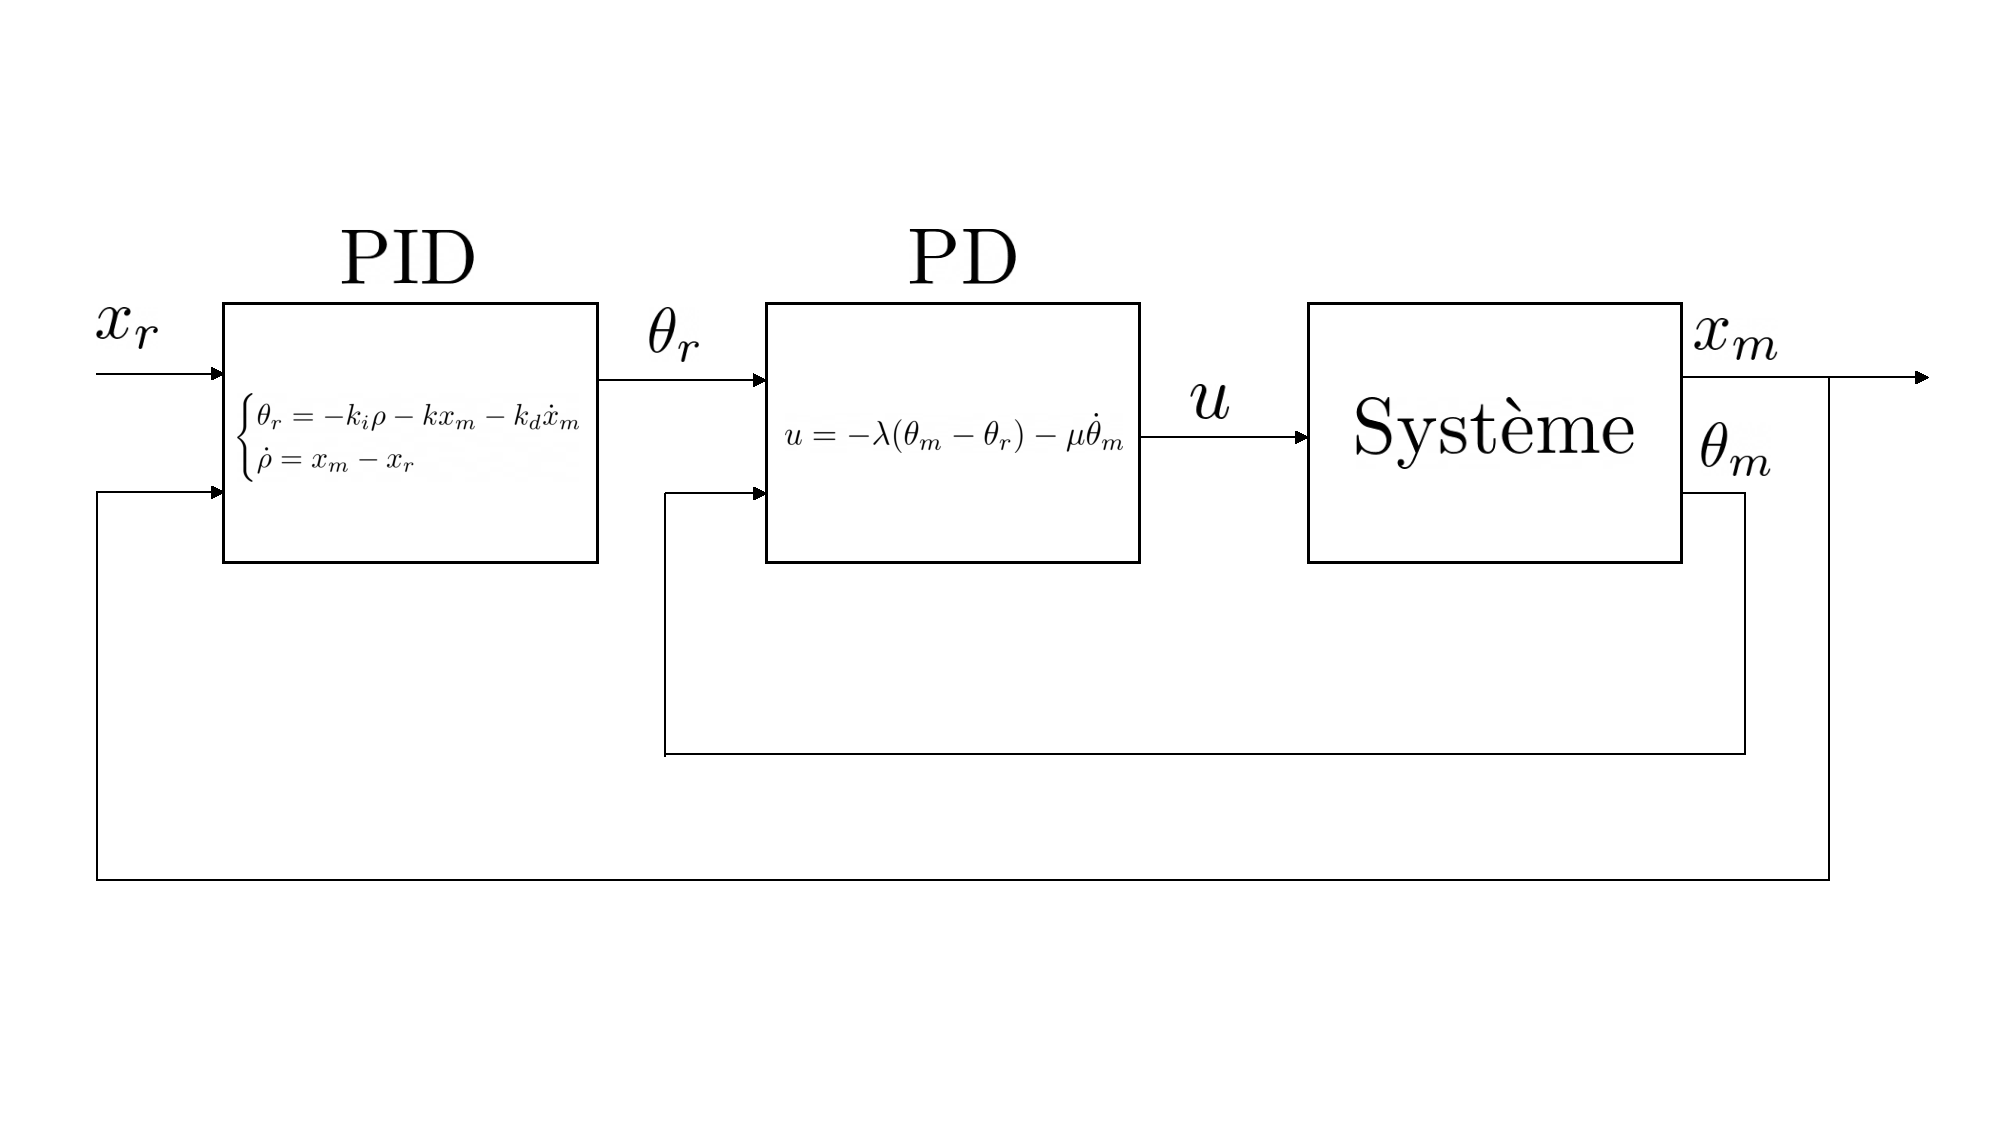
\includegraphics[width=\linewidth]{schemaPD+PID.pdf}
	\caption{Architecture du système bouclé}
\end{figure}

\subsection*{Paramétrage du système rapide}

\noindent En négligeant toujours les bruits de mesure, le système rapide vérifie :

\[
	\begin{cases}
		\dot \theta = q \\
		\dot q =
		\frac{gx \cos \theta - \lambda ( \theta + k_i \rho + k x + k_d v ) - \mu q + d - 2xqv}{\alpha + x^2}
	\end{cases}
\]

\noindent Cela donne le linéarisé, en notant $\gamma = \frac{1}{\alpha + \bar x^2} > 0$ :

\[
	\begin{bmatrix}
		\delta \dot \theta \\
		\delta \dot q
	\end{bmatrix}
	=\begin{bmatrix}
		0 & 1 \\
		- \gamma \lambda & - \gamma \mu
	\end{bmatrix}
	\begin{bmatrix}
		\delta \theta \\
		\delta q
	\end{bmatrix} +
	B_x \delta x +
	B_v \delta v +
	B_\rho \delta \rho +
	B_d \delta d
\]

\noindent Puis le polynôme caractéristique :

\[
	\begin{vmatrix}
		X & -1 \\
		\gamma \lambda & X + \gamma \mu
	\end{vmatrix}
	= X^2 + \gamma \mu X + \gamma \lambda
\]

\noindent D'après le critère de Routh, le système rapide est donc stable si $\lambda > 0$ et $\mu > 0$. On souhaite
imposer un temps de réponse de $0,1 s$. On se propose d'identifier le polynôme caractéristique précédent avec
$X^2 + 2 \xi \omega_0 X + \omega_0^2$ où $\omega_0 = \frac{2 \pi}{0,1} = 20 \pi$ et $\xi = \frac{\sqrt 2}{2}$.
Alors :

\begin{align}
	\lambda &= \frac{\omega_0^2}{\gamma} = \frac{(20 \pi)^2}{\gamma} > 0 \notag \\
	\mu &= \frac{20 \sqrt 2 \pi}{\gamma} > 0 \notag
\end{align}

\noindent Le critère de Routh est bien vérifié par ce paramétrage du système rapide.

\subsection*{Paramétrage du système lent}

\noindent La branche d'équilibre est donnée par : $\delta q= \delta \dot q = 0$. D'où :

\begin{align}
	0 &= \gamma \left[ g \delta x + \delta d - \lambda ( \delta \theta + k_i \delta \rho + k \delta x + k_d \delta v )
	- \mu \delta q \right] \notag \\
	\lambda \delta \theta &= g \delta x + \delta d - \lambda k_i \delta \rho - \lambda k \delta x - \lambda k_d \delta v \notag 
\end{align}

\noindent Le système lent est d'autre part régi par :

\[
	 \begin{cases}
	 	\dot x = v \\
		\dot v = g \sin \theta + x q^2 \\
		\dot \rho = x - x_r
	\end{cases}
\]

\noindent Donc en notant $\eta = \delta \rho$ :

\[
	\begin{bmatrix}
		\delta \dot x \\
		\delta \dot v \\
		\dot \eta
	\end{bmatrix}
	= \begin{bmatrix}
		\delta v \\
		g \delta \theta \\
		\delta x - \delta x_r
	\end{bmatrix}
	= \begin{bmatrix}
		0 & 1 & 0 \\
		g ( \frac{g}{\lambda} - k ) & - g k_d & - g k_i \\
		1 & 0 & 0
	\end{bmatrix} +
	B'_d \delta d + B'_r \delta x_r
\]

\[
	\begin{vmatrix}
		X & - 1 & 0 \\
		g ( k - \frac{g}{\lambda} ) & X + g k_d & g k_i \\
		- 1 & 0 & X
	\end{vmatrix}
	= X^3 + g k_d X^2 + g ( k - \frac{g}{\lambda} ) X + g k_i
\]

\vspace{10px}

\noindent Le critère de Routh donne donc pour condition à la stabilité que $k_d > 0$, $k_i > 0$ et
$g k_d ( k - \frac{g}{\lambda} )  > k_i$. On identifie alors avec le transfert standard
$s^3 + \sigma \sqrt 6 s^2 + \sigma^2 \sqrt 6 s + \sigma^3$ en vérifiant que cela permet toujours de vérifier les
inégalités précédentes. Cela donne :

\begin{align}
	&k_d = \frac{\sigma \sqrt 6}{g} \notag \\
	&k = \frac{\sigma^2 \sqrt 6}{g} + \frac{g}{\lambda} \notag \\
	&k_i = \frac{\sigma^3}{g} \notag
\end{align}

\noindent Les deux premières inégalités sont clairement vérifiées avec $\sigma > 0$. De même pour la dernière,
en effet, dans ces conditions :

\[
	g^2 k_d ( k - \frac{g}{\lambda} )  - g k_i = ( \sigma \sqrt 6 ) ( \sigma^2 \sqrt 6 ) - \sigma^3 = 5 \sigma^3 > 0
\]

\subsection*{Conclusion sur la question 2}

\fbox{
	\begin{minipage}{0.96\textwidth}
		On a bien les systèmes lents et rapides stables. En prenant $\sigma = 3,42$,
		on a alors une réponse temporelle de l'ordre de $1$ seconde.
	\end{minipage}
}

\subsection*{Implémentation Simulink}

\subsubsection*{Approximation des dérivées}

\noindent Afin d'obtenir une version implémentable du contrôleur, on remplace les deux termes dérivés par
leur approximation filtrée. On pose $T_1 =\frac{k_d}{k}$ et $T_2 = \frac{\mu}{\lambda}$. On prend $\varepsilon = \inv{n}$
et on remplace donc $k_d \delta \dot x = k T_1 \delta \dot x$ et
$\mu \delta \dot \theta = \lambda T_2 \delta \dot \theta$ comme suit :

\[
	\begin{bmatrix}
		\dot \eta_x \\
		\dot \eta \\
		\delta \theta_r
	\end{bmatrix}
	= \begin{bmatrix}
		\frac{\delta x - \eta_x}{\varepsilon T_1} \\
		\delta x - \delta x_r \\
		- k_i \eta - k \delta x - k \frac{\delta x - \eta_x}{\varepsilon}
	\end{bmatrix}
	= \begin{bmatrix}
		\frac{n}{T_1} ( \delta x - \eta_x ) \\
		\delta x - \delta x_r \\
		- k_i \eta - k (1 + n) \delta x + k n \eta_x
	\end{bmatrix}
\]
\[
	\begin{bmatrix}
		\dot \eta_\theta \\
		\delta u
	\end{bmatrix}
	= \begin{bmatrix}
		\frac{\delta \theta - \eta_x}{\varepsilon T_2} \\
		- \lambda ( \delta \theta - \delta \theta_r ) - \lambda \frac{\delta \theta - \eta_x}{\varepsilon}
	\end{bmatrix}
	= \begin{bmatrix}
		\frac{n}{T_2} ( \delta \theta - \eta_\theta ) \\
		- \lambda ( 1 + n ) \delta \theta + \lambda \delta \theta_r + \lambda n \eta_\theta
	\end{bmatrix}
\]

\vspace{10px}

\noindent Respectivement pour le contrôleur PD et pour le PID. On va alors prendre $n = 20$ pour approximer au mieux
la dérivée. 

\subsubsection*{Passage aux différences finies}

\noindent On peut réécrire le jeux d'équations :

\[
	\begin{cases}
		\dot \eta_x = \frac{n}{T_1} ( \delta x - \eta_x ) \\
		\dot \eta = \delta x - \delta x_r \\
		\dot \eta_\theta = \frac{n}{T_2} ( \delta \theta - \eta_\theta ) \\
		\delta u = - \lambda ( 1 + n ) \delta \theta - \lambda k_i \eta -  \lambda k (1 + n) \delta x +
		\lambda k n \eta_x + \lambda n \eta_\theta
	\end{cases}
\]

\noindent On remplace maintenant les termes en $\delta$ par les différences finies : $\delta x \to x - \bar x$,
$\delta x_r \to x_r - \bar x$, $\delta \theta \to \theta - \bar \theta$ et $\delta u = u - \bar u$.

\[
	\begin{bmatrix}
		\dot \eta_x \\
		\dot \eta \\
		\dot \eta_\theta \\
		u - \bar u
	\end{bmatrix}
	= \begin{bmatrix}
		\frac{n}{T_1} ( x - \bar x - \eta_x ) \\
		x - x_r \\
		\frac{n}{T_2} ( \theta - \bar \theta - \eta_\theta ) \\
		- \lambda ( 1 + n ) ( \theta - \bar \theta ) - \lambda k_i \eta - \lambda k (1 + n) ( x - \bar x ) +
		\lambda k n \eta_x + \lambda n \eta_\theta
	\end{bmatrix}
\]

\noindent On pose  $\mu_i = \eta + \inv{\lambda k_i} \left( \bar u +
\lambda (1 + n) \bar \theta + \lambda k (1 + n) \bar x - \lambda k n \bar x -
\lambda k n \bar \theta \right)$, $\mu_x = \eta_x + \bar x$ et $\mu_\theta = \eta_\theta + \bar \theta$.

\noindent On obtient finalement le contrôleur implémentable suivant :

\[
	\begin{bmatrix}
		\dot \mu_x \\
		\dot \mu_i \\
		\dot \mu_\theta \\
		u
	\end{bmatrix}
	= \begin{bmatrix}
		\frac{n}{T_1} ( x - \mu_x ) \\
		x - x_r \\
		\frac{n}{T_2} ( \theta - \mu_\theta ) \\
		- \lambda ( 1 + n ) \theta - \lambda k_i \mu_i - \lambda k (1 + n) x + \lambda k n \mu_x + \lambda n \mu_\theta
	\end{bmatrix}
\]

\vspace{10px}

\noindent On note $X = (\mu_x, \mu_i, \mu_\theta)$, $U = (x, \theta, x_r)$ et $Y = u$. Alors le contrôleur est donné par :

\[
	\begin{cases}
		\dot X =
		\underbrace{
		\begin{bmatrix}
			- \frac{n}{T_1} & 0 & 0 \\
			0 & 0 & 0 \\
			0 & 0 & - \frac{n}{T_2}
		\end{bmatrix}
		}_{M} X +
		\underbrace{
		\begin{bmatrix}
			\frac{n}{T_1} & 0 & 0 \\
			1 & 0 & -1 \\
			0 & \frac{n}{T_2} & 0
		\end{bmatrix}
		}_{N} U \\
		Y = \underbrace{
		\begin{bmatrix}
			\lambda k n &  - \lambda k_i & \lambda n
		\end{bmatrix}
		}_{P} X +
		\underbrace{
		\begin{bmatrix}
			- \lambda k (1 + n) &- \lambda (1 + n) & 0
		\end{bmatrix}
		}_{Q} U
	\end{cases}
\]

\subsubsection*{Conditions intiales}

\noindent On suppose enfin que l'on part d'un point d'équilibre. On prend donc les conditions initiales suivantes :

\[
	X_{t = 0} = \begin{bmatrix}
		\mu_x (t = 0) \\
		\mu_i (t = 0) \\
		\mu_\theta (t = 0)
	\end{bmatrix}
	= \begin{bmatrix}
		\bar x \\
		\frac{-1}{k_i} ( k \bar x + \bar \theta +\frac{\bar u}{\lambda}  ) \\
		\bar \theta
	\end{bmatrix}
\]

\subsection*{Conclusion sur la question 3}

\noindent Si on prend enfin la condition intiale $X = \bar X$ correspondant au point d'équilibre associé à $\bar x = 0$
et $x_r = 0,4 m$ de sorte que la bille parcoure $40 cm$, on a les résultats graphiques suivants :

\begin{figure}[H]
	\centering
	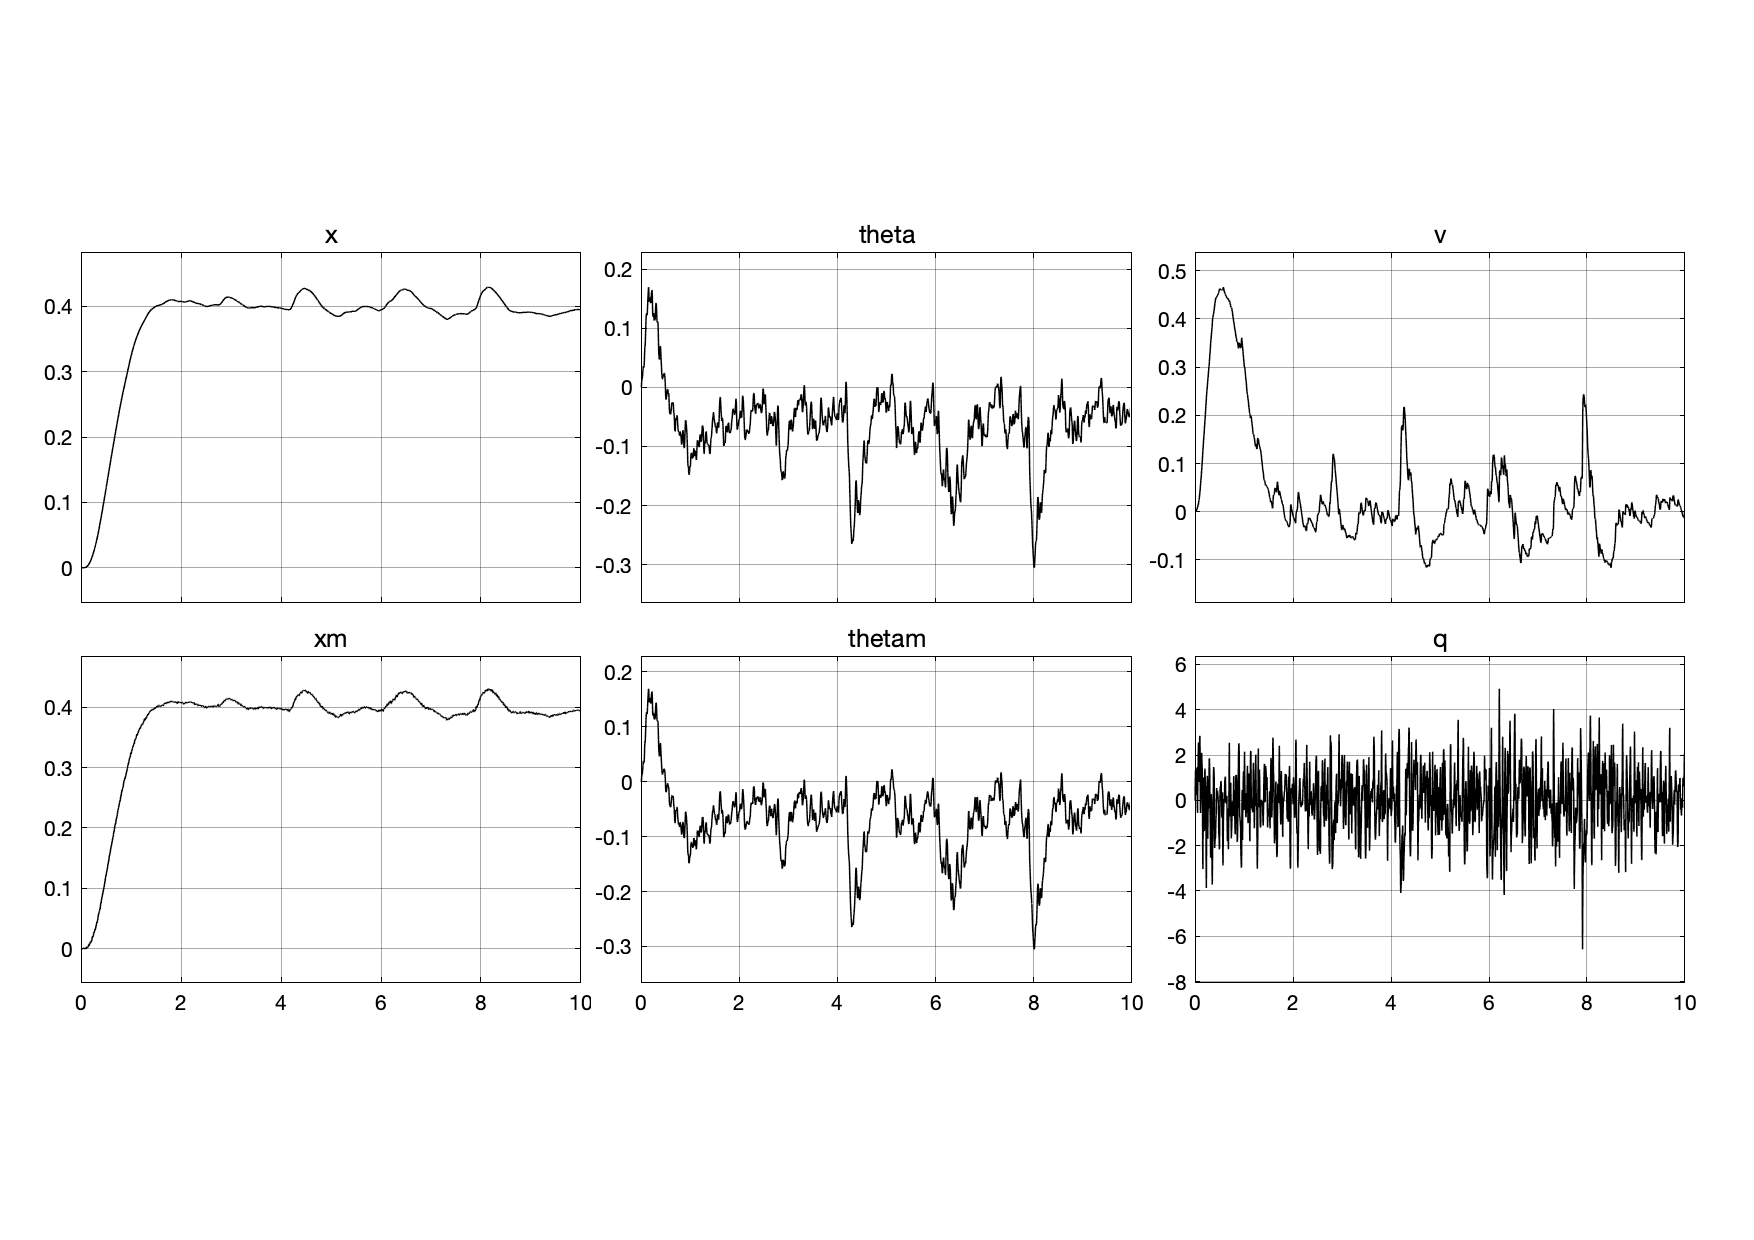
\includegraphics[width=\linewidth]{resultat.pdf}
	\caption{Réponse à une consigne constante}
\end{figure}

\noindent La bille parcourt bien $40cm$ mais tombe en réalité du rail car $x$ dépasse $0,4m$.

\vspace{10px}

\noindent \fbox{
	\begin{minipage}{0.96\textwidth}
		Afin que la bille parcoure bien $40cm$ sans tomber du rail, on garde les mêmes conditions initiales et on prend
		les consignes suivantes qui répondent au problème :
		\begin{itemize}
			\item Un échelon de valeur initiale $-0,3m$ et de valeur finale $0,3m$
			\item Une consigne sinusoïdale de phase et de biais nuls et d'amplitude $0,6m$
			\item Une rampe de valeur initiale $-0,3m$.
		\end{itemize}
		On a représenté les différents résultats sur les graphes qui suivent.
	\end{minipage}
}

\begin{figure}[H]
	\centering
	\includegraphics[width=\linewidth]{step.pdf}
	\caption{Réponse à une consigne en échelon}
\end{figure}

\begin{figure}[H]
	\centering
	\includegraphics[width=\linewidth]{sine.pdf}
	\caption{Réponse à une consigne sinusoïdale}
\end{figure}

\begin{figure}[H]
	\centering
	\includegraphics[width=\linewidth]{ramp.pdf}
	\caption{Réponse à une rampe}
\end{figure}

\end{document}










